\chapter{Analytical solutions of the Landau-Lifshitz-Gilbert equation}
\chaptermark{Analytical solutions}
\label{cha:analyt-solut-land}

When testing numerical methods for differential equations it is very helpful to be able to compare the results with known analytical solutions.
\Thisref{cha:analyt-solut-land} contains some solutions useful for this purpose.

\section{Ellipsoidial nano-particle solution}

In a 2000 paper \cite{Mallinson2000} Mallinson gives an analytical equation for the time taken for magnetisation to ``switch'' from one polar angle (angle to the field axis) to another.
He also gives the azimuthal angle (the angle around the field axis) rotated through during this switching.

The conditions for this model to apply are:
\begin{enumerate}
\item Constant applied field.
\item ``Infinite'' exchange field (\ie particle is sufficiently small that the exchange field dominates and the magnetisation is uniform).
\item Uniaxial anisotropy.
\item Prolate ellipsoidal particle (to have a simple analytical magnetostatic field)
\item All effective fields along the same axis.
\end{enumerate}

Let $\theta_1$, $\theta_2$ be the initial and final angles between the field axis and the magnetisation (\ie initial and final polar angles in the spherical polar coordinate system with the field axis as the main axis).
Let $H_k$ be the combined anisotropy field: $H_k = \frac{2 K}{M_s} + M_s(N_\perp - N_\parallel)$ where $N$ is the demagnetisation tensor of the ellipsoid.
All other symbols have their usual meanings.
Then the time taken to switch from $\theta_1$ to $\theta_2$ is
\begin{equation}
  \tau = \frac{\dampc^2 +1}{\gymagc \dampc} \frac{1}{H^2 - H_k^2}
  \bigb{ H \ln \bigs{ \frac{\tan(\theta_2/2)}{\tan(\theta_1/2)} }
       + H_k \ln \bigs{ \frac{H - H_k \cos\theta_1}{H - H_k \cos\theta_2} }
       + H_k \ln \bigs{ \frac{\sin\theta_2}{\sin\theta_1} }
     }.
\label{eq:80}
\end{equation}

The azimuthal angle precessed through during this switching is
\begin{equation}
  \phi = \frac{-1}{\dampc} \ln \bigs{ \frac{\tan(\theta_2/2)}{\tan(\theta_1/2)} }.
\end{equation}

Note that this is not really a true analytical solution to the Landau-Lifshitz-Gilbert equation:
it gives the switching time and azimuthal angle as a function of polar angle rather than the magnetisation direction as a function of time.
However comparing switching time values with those generated by a model is still a useful measure of the error.
Additionally the magnetisation at some given time could be calculated from \cref{eq:80} using \eg the Newton-Raphson method.
Alternatively, using further simplifying assumptions, this solution can be reduced to a ``true'' analytical solution in the sense that $\mv$ can be written analytically as a function of time.
This is discussed in \cref{sec:aimr-llg-problem-definition}.


\section{Wave-like solution in an infinite domain}
\label{sec:wave-like-solution}

These solutions are taken from \cite{Jeong2014}, \cite{Fuwa2006}, the solution appears to have been originally published in \cite{Lakshmanan1976} in a more abstract form.
For most parameters the solution is just a wave-like excitation in $m_x(\xv, t)$ and $m_y(\xv, t)$ whose oscillations are damped towards a uniform $m_z = \pm 1$ state over time.
As far as the author is aware this is the only exact solution of the LLG equation with the exchange effective field which has non-trivial $\xv$ dependence.

For an infinite magnetic domain (\ie using periodic boundary conditions) of dimension $D$ choose some constant $c \in \real$ and $\kvec \in \real^D$.
Write
\begin{equation}
  \begin{aligned}
    \that(t) &= \frac{t}{1 + \dampc^2}, \\
    b(t) &= \abs{\kvec}^2 \dampc \that(t), \\
    d(t) &= \sqrt{\sin^2(c) + \cos^2(c)e^{2 b(t)}}, \\
    g(t) &= \frac{1}{\dampc} \log \bigs{ \frac{d(t) + \cos(c) e^{b(t)}}{1 + \cos(c)} }.
  \end{aligned}
\end{equation}
Then
\begin{equation}
  \begin{aligned}
    m_x(t) &= \frac{1}{d(t)} \sin(c) \cos\bigb{\kvec \cdot \xv + g(t) }, \\
    m_y(t) &= \frac{1}{d(t)} \sin(c) \sin\bigb{\kvec \cdot \xv + g(t) }, \\
    m_z(t) &= \frac{1}{d(t)} \cos(c) e^{b(t)},
  \end{aligned}
\end{equation}
is a solution of the Landau-Lifshitz-Gilbert equation with $\heff = \lap \mv$.

The rescaling of time given by $\that(t)$ is needed to convert from a solution of the Landau-Lifshitz equation \cref{eq:ll-nd-simpler} to a solution of the Landau-Lifshitz form of the Landau-Lifshitz-Gilbert equation \cref{eq:ll-nd-llglike}, \ie to account for the correction to the form of the damping as introduced by Gilbert.

The function $d(t)$ is a normalisation parameter to keep $\abs{\mv(\xv, t)} = 1$ everywhere.
To see this: note that $\sin^2(c) \cos^2\bigb{f(\xv)} + \sin^2(c) \sin^2\bigb{f(\xv)} = \sin^2(c)$, hence the length contribution of the combined $x$ and $y$ terms is $\sin^2(c)$.

The vector $\kvec$ is the wave vector, it determines the direction and speed of propagation of the wave.

The parameter $c$ represents in some way the fraction of the initial magnetisation which takes part in the oscillations.
If $c = 0$ then $m_x, m_y = 0$ and there is no wave.

\begin{figure}
  \centering
  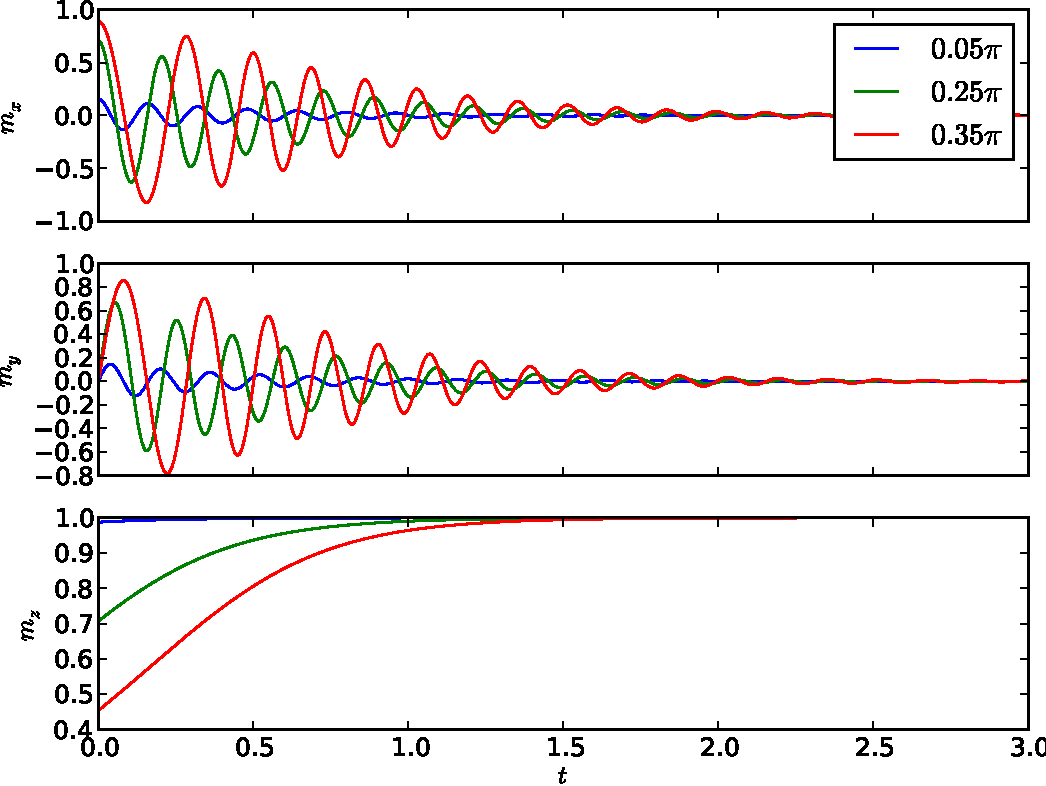
\includegraphics[width=0.8\textwidth]{plots/wave_exact_solution_parameters/exact_solution_parameters.pdf}
  \caption{One dimensional wave solution values over time at $x=0$ with $k = 2\pi$, $\dampc = 0.05$ and various $c$ well away from $\frac{\pi}{2}$.}
  \label{fig:wave-solution-vary-c}
\end{figure}

\Cref{fig:wave-solution-vary-c} shows the solution in one dimension over time at $\xv = 0$ with parameters $k = 2\pi$, $\dampc = 0.05$ and varying $c$.
As $c$ increases the initial value of $m_z$ decreases and the amplitude of the oscillations in $m_x$ and $m_y$ increase.

As $c$ approaches $\frac{\pi}{2}$ the behaviour becomes more complex, this is shown in \cref{fig:wave-solution-vary-c-complex}.
Essentially there is an additional initial exponential decay towards a state with moderate $m_z$ after which the dynamics are similar to the case for lower $c$.
At $c=\frac{\pi}{2}$ then $\mv(\xv, t)= (\cos(\kv\cdot\xv), \sin(\kv\cdot\xv), 0)$ and there are no dynamics.
Above $c=\frac{\pi}{2}$ the initial $m_z$ goes negative and the behaviour is symmetrical with that below $c=\frac{\pi}{2}$

\begin{figure}
  \centering
  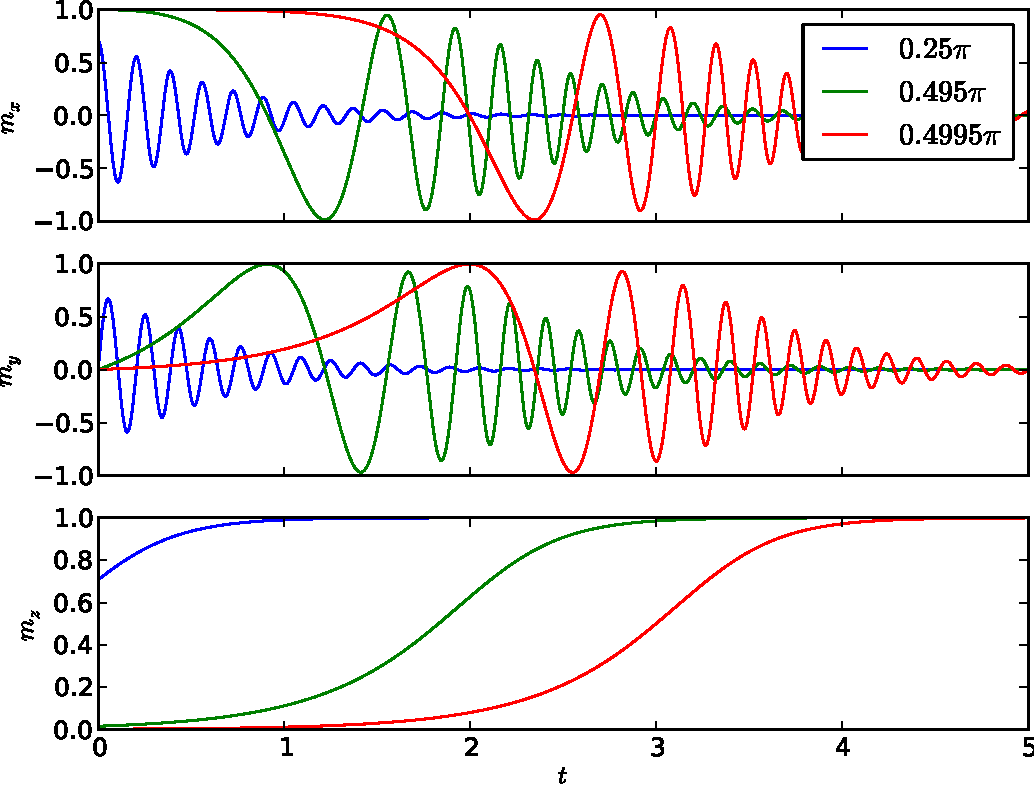
\includegraphics[width=0.8\textwidth]{plots/wave_exact_solution_parameters/exact_solution_parameters_complex.pdf}
  \caption{One dimensional wave solution values over time at $x=0$ with $k = 2\pi$, $\dampc = 0.05$ and $c$ approaching the critical value $\frac{\pi}{2}$.}
  \label{fig:wave-solution-vary-c-complex}
\end{figure}


In the limit of $\dampc \goesto 0+$ the solution becomes \cite{Fuwa2006}:
\begin{equation}
  \begin{aligned}
    m_x &= \sin(c) \cos\bigb{\kvec \cdot \xv + \abs{\kvec}^2 \cos(a) t}, \\
    m_y &= \sin(c) \sin\bigb{\kvec \cdot \xv + \abs{\kvec}^2 \cos(a) t}, \\
    m_z &= \cos(c).
  \end{aligned}
\end{equation}
This is just a simple wave in space and time.

Note that the behaviour in higher dimensions is essentially the same as the 1D behaviour shown here except that the direction of propagation is in the direction described by the vector $\kv$.





%%% Local Variables:
%%% mode: latex
%%% TeX-master: "main"
%%% End:
